\documentclass[10pt,letterpaper]{article}

\usepackage{ccn}
\usepackage{pslatex}
\usepackage{svg}
\usepackage{apacite}
\usepackage{amsmath}
\usepackage{graphicx}

\title{How much do we know about visual representations? \\Quantifying the dimensionality gap between DNNs and visual cortex}

\author{
    {\large \bf Raj Magesh Gauthaman (rgautha1@jh.edu)} \\
    Department of Cognitive Science, Johns Hopkins University\\
    3400 N Charles Street, Baltimore, MD 21218, United States
    \AND
    {\large \bf Michael F Bonner (mbonner5@jh.edu)} \\
    Department of Cognitive Science, Johns Hopkins University\\
    3400 N Charles Street, Baltimore, MD 21218, United States
}

\begin{document}

\maketitle

\section{Abstract}
{
\bf
Deep neural networks (DNNs) can explain a large portion of variance in image-evoked cortical responses by accounting for the highest variance latent dimensions in neural data, such as dimensions corresponding to animacy, aspect ratio, and curvature. However, there is a long tail of low-variance latent dimensions in image-evoked cortical responses that may nonetheless be critical to human vision. We wondered if these low-variance dimensions are meaningful and whether current DNNs are successful in explaining them. To answer these questions, we estimated the number of reliable dimensions in visual cortex in a large-scale human fMRI dataset and assessed how well DNNs performed at explaining these dimensions. We found that hundreds of dimensions contained reliable stimulus-relevant information. However, standard DNN encoding models explain a much smaller number of these dimensions\textemdash often an order of magnitude smaller than the number of reliable dimensions in the data. Our findings demonstrate the surprisingly low-dimensional nature of explained variance in computational models of visual cortex, and reveal the long-tail of complex, stimulus-relevant information in cortical responses that remains to be explained.
}

\begin{quote}
    \small
    \textbf{Keywords:} 
    fMRI; dimensionality; DNN; encoding models; visual cortex
\end{quote}

\section{Introduction}

Image-evoked cortical responses to natural images have rapidly decaying eigenspectra, where a large fraction of their variance is captured by relatively few dimensions, including those corresponding to animacy, aspect ratio, and curvature. The many remaining low-variance dimensions are more difficult to interpret and are often attributed to stimulus-independent noise. Contrary to this interpretation, recent work has demonstrated that the performance of deep encoding models of visual cortex scales with their latent dimensionality: high-dimensional models predict neural responses better \cite{Elmoznino2021}. High-dimensional representations have been shown to enable efficient few-shot learning of novel concepts in neural systems \cite{Sorscher2021} and such geometry has recently been described in population responses of the mouse visual cortex \cite{Stringer2019}. Together, these observations suggest that the dimensionality of image-evoked responses in primate visual cortex might be higher than previously estimated \cite{Haxby2011, Lehky2014}.

State-of-the-art computational models of the visual cortex explain most of the variance in neural responses to natural images. However, since most of this variance is driven by a small number of high-variance dimensions, a model that predicts only these dimensions while neglecting the long tail of low-variance dimensions would nevertheless "successfully" explain much of the variance in neural data. Whether current computational models of the visual cortex explain all the reliable dimensions in neural responses or achieve their impressive performance by simply explaining a few high-variance dimensions remains unclear.

In this study, we estimate the number of meaningful latent dimensions in image-evoked cortical responses using the large-scale Natural Scenes human fMRI dataset \cite{Allen2021}, and we demonstrate that the latent dimensionality is significantly higher than previously reported. We then investigate whether standard deep neural network models of visual cortex successfully explain all these dimensions and find a significant gap between the dimensionalities of the model and the brain, suggesting that evaluating encoding models using explained variance might inflate their apparent similarity to human visual representations.

\begin{figure*}[ht]
    \centering
    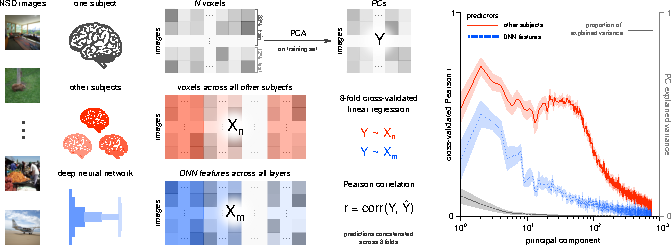
\includegraphics[width=1\textwidth]{ccn}
    \caption[width=1\textwidth]{Computational models of the visual cortex fail to explain most reliable dimensions in high-dimensional neural data. (Left) The principal components $Y$ of cortical responses to images in the Natural Scenes Dataset are predicted using cross-validated linear regression with either neural responses from other subjects ($X_n$, neural predictors) or image-computable deep neural network features ($X_m$, model predictors). (Right) More principal components of the neural data are reliably predicted by the neural predictors (red) compared to the model-based predictors (blue), revealing a dimensionality gap between the model and the brain. The shaded regions depict standard errors of the mean across 8 subjects.}
    \label{figure-0}
\end{figure*}

\section{Methods}
The Natural Scenes Dataset (NSD) includes fMRI responses from 8 participants who viewed 9,000\textendash 10,000 natural images of scenes while performing a continuous recognition task. We used the 1.8-mm volume preparation of the NSD data with version 3 of the single-trial betas. We restricted our analyses to the $N = 872$ unique images viewed by all 8 participants and only included regions of interest (ROIs) identified using population receptive field mapping or functional localizers, including the ventral and dorsal visual streams and object-, scene-, face-, body- and word-selective regions. We report results obtained by concatenating the voxels in all these ROIs, though similar patterns were observed in each individual region. For each subject $s$, we constructed the $(N \text{ images} \times V_s \text{ voxels})$ activation matrix $A_s$ after computing the mean activation to each image across repetitions.

While many approaches exist to identify latent dimensions in high-dimensional data, we adopted principal component analysis (PCA) for our approach to estimating the number of reliable dimensions. If a principal component of the neural data can be reliably predicted using cross-validated linear regression, it must contain stimulus-relevant information regardless of how much variance lies along that direction. We reasoned that the best general model of the visual cortex can only predict these dimensions as well as they can be predicted from the brains of other subjects.

For each subject $s$, we divided the images into 8 folds, standardized the data $A_s$ using the mean and standard deviation of the training set, and projected it onto the principal components of the training set to obtain an $(N \text{ images} \times P \text{ PCs})$ target matrix $Y_s$ (Figure \ref{figure-0}, top-left). Then, we constructed the $(N \text{ images} \times \sum_{s' \in S, s' \neq s} V_s \text{ voxels})$ neural predictor matrix $X_n$ by concatenating the neural responses of all other subjects (Figure \ref{figure-0}, middle-left). In addition, we extracted image features from all the convolutional and fully connected layers of AlexNet trained on ImageNet \cite{Krizhevsky2012}. The convolutional feature maps were spatially max-pooled, and these features were concatenated with those from the fully connected layers to produce an $(N \text{ images} \times F \text{ features})$ model-derived predictor matrix $X_m$ (Figure \ref{figure-0}, bottom-left). Linear regression was used to predict each of the principal components in the target matrix $Y_s$ using either the neural features $X_n$ or the model-derived features $X_m$. The encoding performance was computed as the Pearson correlation between actual and predicted responses after concatenating across all 8 folds of the data.

\section{Results \& Discussion}
We find a surprisingly large number of dimensions in the neural data that are reliably predicted by the neural predictors, demonstrating the high-dimensional geometry of stimulus-relevant information in cortical responses (Figure \ref{figure-0}, right, solid red). However, we observe that the model-based predictors fail to predict much of the variance in most of these reliable dimensions (Figure \ref{figure-0}, right, dotted blue).

Our finding of high-dimensional geometry in cortical responses is consistent with similar findings in mouse visual cortex, where the dimensionality of the population responses did not exhibit a characteristic scale but instead displayed power-law scaling \cite{Stringer2019}. That such high-dimensional structure is observed even with the coarse spatial scale afforded by functional neuroimaging is encouraging, suggesting that visual representations obtained through fMRI can be effectively used to study the high-dimensional regime with sufficiently large datasets.

Our results also demonstrate that traditional computational models of visual cortex rely on a few high-variance dimensions to achieve good encoding performance but neglect the long tail of reliable low-variance dimensions that contain stimulus-relevant information. We propose that the number of reliably estimated dimensions is an important summary statistic for encoding model performance and gives an insightful, alternative perspective to the average explained variance. In future work, we plan to explore the representational content and the perceptual and behavioral correlates of these low-variance dimensions, which potentially contain fine-grained visual information that is used to perform complex tasks.

\bibliographystyle{apacite}
\setlength{\bibleftmargin}{.125in}
\setlength{\bibindent}{-\bibleftmargin}

\bibliography{references}

\end{document} 
